\subsection{Preventivo a finire}
In seguito al completamento delle fasi relative alla Requirements and Technology Baseline, è emerso che vi è stata una previsione della distribuzione delle ore di lavoro tra l'amministratore e il responsabile sbilanciata, causando un eccesso di ore rimanenti per il responsabile e un deficit di ore rimanenti per l'amministratore al momento della conclusione della \textit{RTB}\textsubscript{\textit{G}}.

Di seguito la tabella delle risorse utilizzate e rimanenti secondo la stima dei costi di realizzazione effettuata in data 16/11/2023~(\textit{\S~\ref{sec:SecondaStesura}}):
\begin{figure}[H]
    \centering
    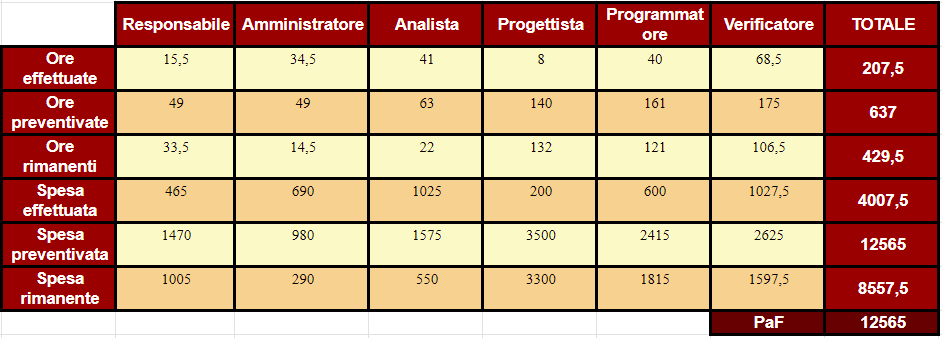
\includegraphics[width=0.8\textwidth]{../Images/PaF1stesura.PNG}
    \caption{Riepilogo risorse utilizzate secondo la seconda stesura dei costi di realizzazione}
    \label{fig:RisorseRimanentiRTB}
\end{figure}

Pertanto, si è deciso di rivalutare le risorse come descritto nella \textit{sezione~\S~\ref{sec:TerzaStesura}}, di seguito la tabella delle risorse utilizzate e rimanenti secondo tale stima.

\begin{figure}[H]
    \centering
    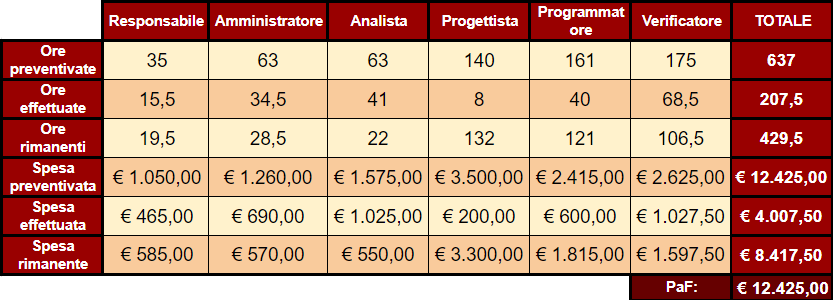
\includegraphics[width=0.8\textwidth]{../Images/PaF2stesura.PNG}
    \caption{Riepilogo risorse utilizzate secondo la terza stesura dei costi di realizzazione}
    \label{fig:RisorseRimanentiRTB2}
\end{figure}    
Il preventivo a finire è ora quindi di \textbf{12425,00€} mentre la consegna finale del prodotto slitta al \textbf{25/03/2024}, per via del tempo dedicato allo studio per gli esami durante il sesto periodo come indicato nella \textit{sezione~\S~\ref{sec:SecondaStesuraCalendario}}.

